\documentclass{beamer}
\mode<presentation>
{
	\usetheme{default}      % or try Darmstadt, Madrid, Warsaw, ...
	\usecolortheme{default} % or try albatross, beaver, crane, ...
	\usefonttheme{default}  % or try serif, structurebold, ...
	\setbeamertemplate{navigation symbols}{}
	\setbeamertemplate{caption}[numbered]
} 

\usepackage[slovene]{babel}
\usepackage{graphicx, amsmath, listings, amssymb, commath, float}
\usepackage[utf8]{inputenc}
\usepackage[section]{placeins}

\title{Presek dveh implicitno danih ploskev}
\author[Avtorji]{Aljaž Verlič, Blažka Blatnik, Lina Lumburovska, Luka Tavčer\\
	Mentor: Damir Franetič}
\date{5. junij 2017}
\begin{document}
	
	\begin{frame}
		\titlepage
	\end{frame}
	
	\begin{frame}{Opis problema}
		V $\mathbb{R}^3$ imamo podani dve poljubni implicitno dani ploskvi, opisanimi z enačbama $f_{1}(x)$ = $C_{1}$ in $f_{2}(x)$ = $C_{2}$.\\
		Naša naloga je poiskati krivuljo $K$, ki predstavlja presek teh dveh ploskev.\\
		\vspace{5mm}
		Presek ploskev je množica rešitev nelinearnega sistema enačb:
		\begin{center}
			$f_{1}(x)$ = $C_{1}$\\$f_{2}(x)$ = $C_{2}$
		\end{center}
	\end{frame}
	
	\begin{frame}{Opis modela}
		Sistem lahko gledamo tudi, kot enačbe nivojnic funkcij  $f_{1}$ in $f_{2}$, krivulja K pa je presek teh nivojnic. Gradienta funkcij sta tako v vsaki točki krivulje preseka, pravokotna nanjo. To opišemo:
		\begin{center}
			$F(x) = \dfrac{(grad f_{1}(x))x (grad f_{2}(x))}{\|grad f_{1}(x))x (grad f_{2}(x))\|}$
		\end{center}
		in označimo $x = x(t)$ naravno parametrizacijo krivulje K. Ta x je rešitev avtonomnega sistema diferencialnih enačb:
		\begin{center}
			$\dot{x} = F(x)$
		\end{center}
	\end{frame}
	
	\begin{frame}{Opis metod}
		Za reševanje sistema $\dot{x} = F(x)$ lahko uporabimo katero izmed numeričnih metod za reševanje diferencialnih enačb:
		\begin{itemize}
			\item Eulerjeva metoda
			\begin{itemize}
				\item Bolj logična in preprosta
				\item Komulativna napaka z vsakim korakom narašča
			\end{itemize}
			\item Runge-Kutta 4. reda
			\begin{itemize}
				\item Bolj natančna
				\item Napaka precej manjša, kot pri Eulerjevi metodi
			\end{itemize}
		\end{itemize}
	\end{frame}
	
	\begin{frame}{Eulerjeva metoda}
		\begin{itemize}
			\item Na vsakem koraku naslednjo točko $(x_{i+1},y_{i+1})$ dobimo tako, da se za h (korak) premaknemo vzdolž tangente na rešitev $(x_{i},y_{i})$. 
			\item Točka $(x_{i+1},y_{i+1})$ leži na drugi partikularni rešitvi kot $(x_{i},y_{i})$.
			\item Napaka na vsakem koraku je reda $O(h^2)$.
		\end{itemize}
		\begin{block}{Geometrijsko:}
			\begin{figure}
				\centering
				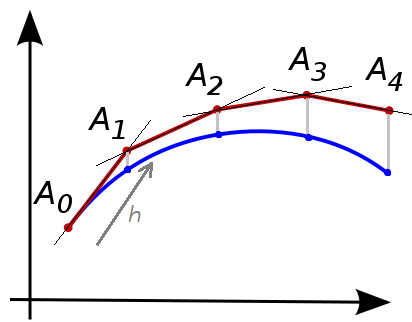
\includegraphics[width=0.55\textwidth]{Euler_method_geom}
			\end{figure}
		\end{block}
	\end{frame}
	
	\begin{frame}{Eulerjeva metoda brez popravljanja}
		Opazimo, da je Eulerjeva metoda brez popravljanja približka "blizu" pravilni rešitvi, vendar se napaka z iteracijami povečuje. \\
		\begin{center}
			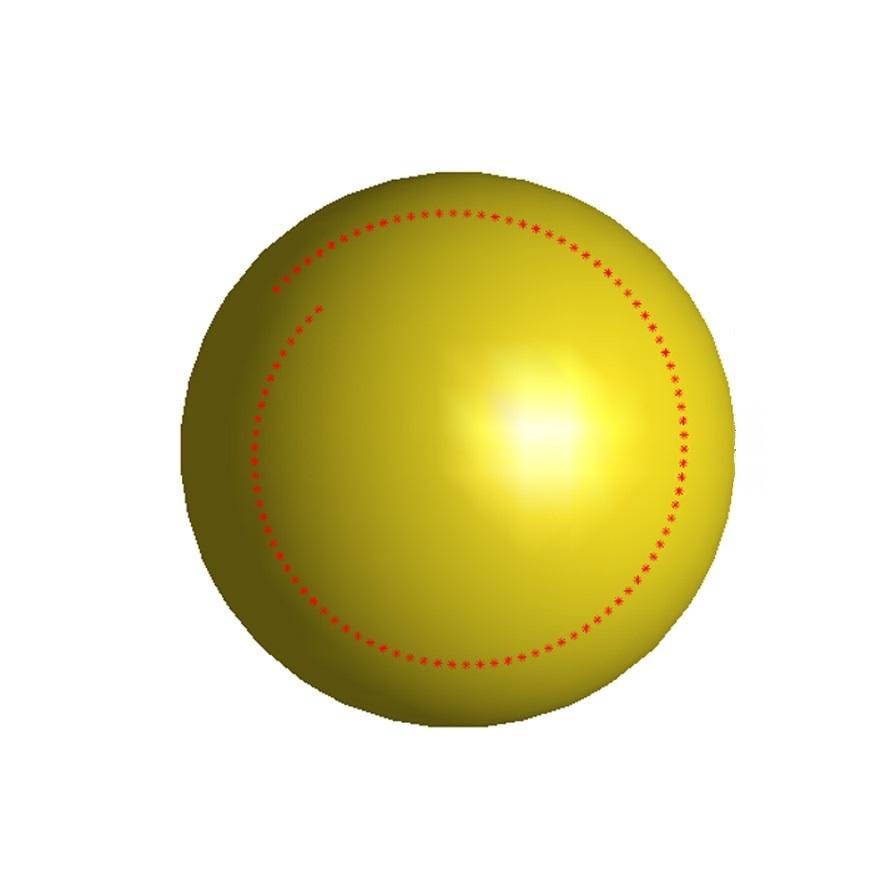
\includegraphics[scale=0.30]{eul1}
		\end{center}
	\end{frame}
	
	\begin{frame}{Eulerjeva metoda brez popravljanja}
		Napake, ki se seštevajo, so na večjem intervalu bolj opazne.\\
		\begin{center}
			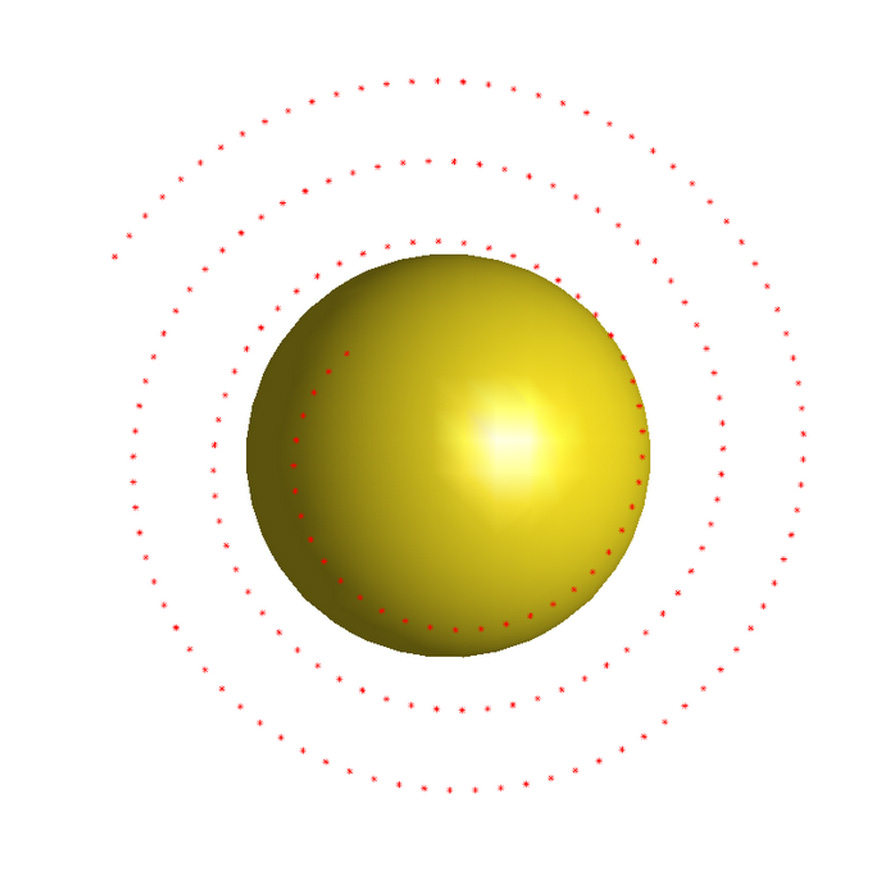
\includegraphics[scale=0.30]{eul2}
		\end{center}	
	\end{frame}
	
	\begin{frame}{RK4 metoda}
		Natančnost se izboljša, če za izračun začetnih približkov uporabimo Runge-Kutta reda 4, a še vedno ne dovolj, zato moramo tudi tu za popravljanje uporabiti Newtonovo metodo.
		
		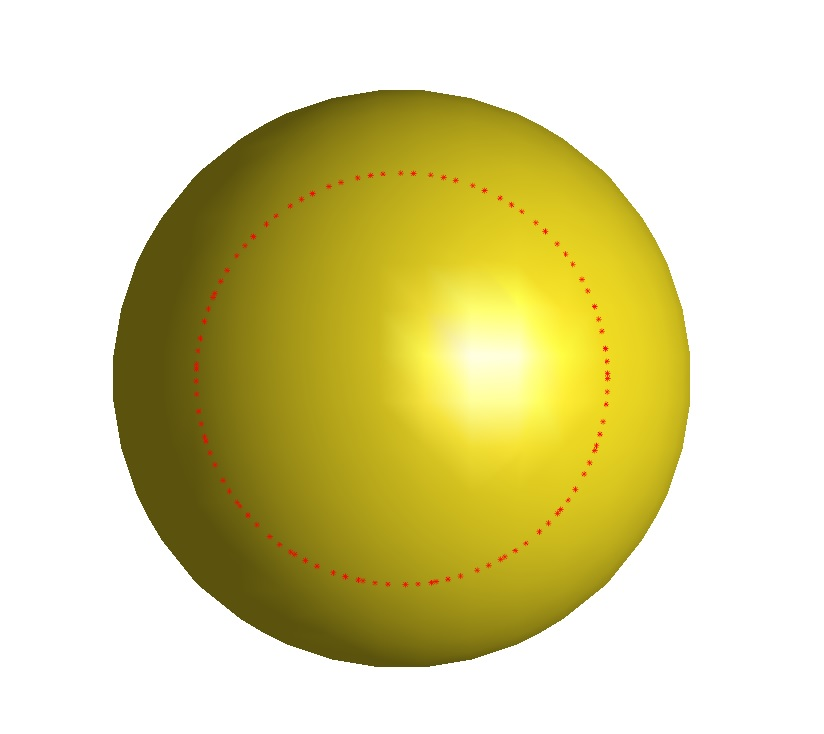
\includegraphics[scale=0.30]{rk4}
		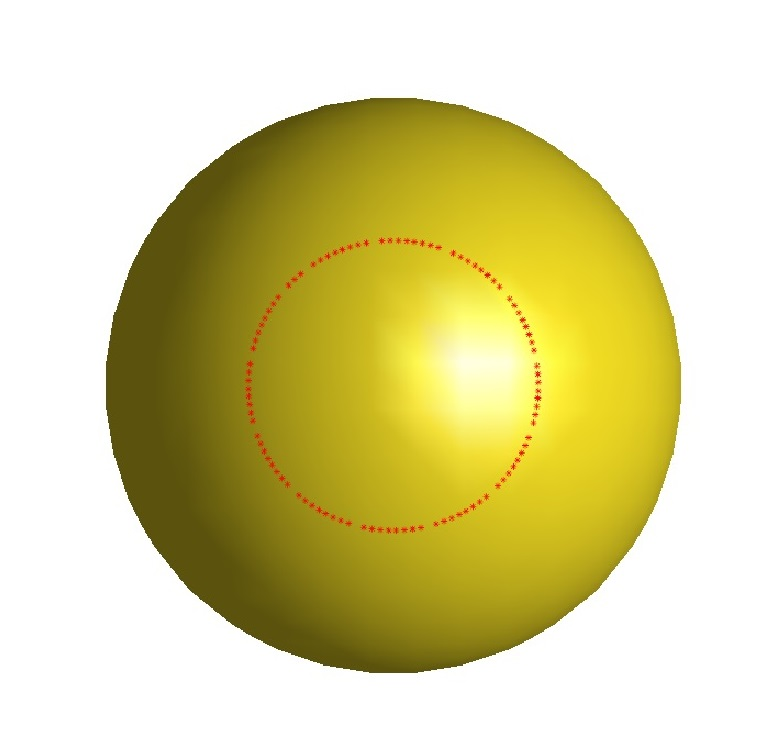
\includegraphics[scale=0.30]{rk4_newt}
		
	\end{frame}
	
	\begin{frame}{Newtonova metoda za popravljanje približka}
		\begin{itemize}
			\item Z opisanima metodama za reševanje DE enačb, dobimo na vsakem koraku le približek (Posebej razvidno iz Eulerjeve metode).
			\item Približek želimo popraviti tako, da bo spet ležal na krivulji preseka.
		\end{itemize}
		Dobljeni približek y, želimo popraviti na nek x, ki bo ležal na preseku. Če zapišemo $F(y) \cdot x = F(y)\cdot y $, nam to predstavlja enačbo ravnine, ki je zelo blizu normalni ravnini na krivuljo K. Z Newtonovo metodo z začetnim približkom y rešimo sistem enačb:
		\begin{center}
			$f_{1}(x)$ = $C_{1}$\\$f_{2}(x)$ = $C_{2}$\\ $F(y) \cdot x = F(y)\cdot y $
		\end{center}
	\end{frame}
	
	\begin{frame}{Eulerjeva metoda s popravljanjem z Newtonovo metodo}
		Ko za popravljanje napake uporabimo Newtonovo metodo, dobimo pravilno rešitev.
		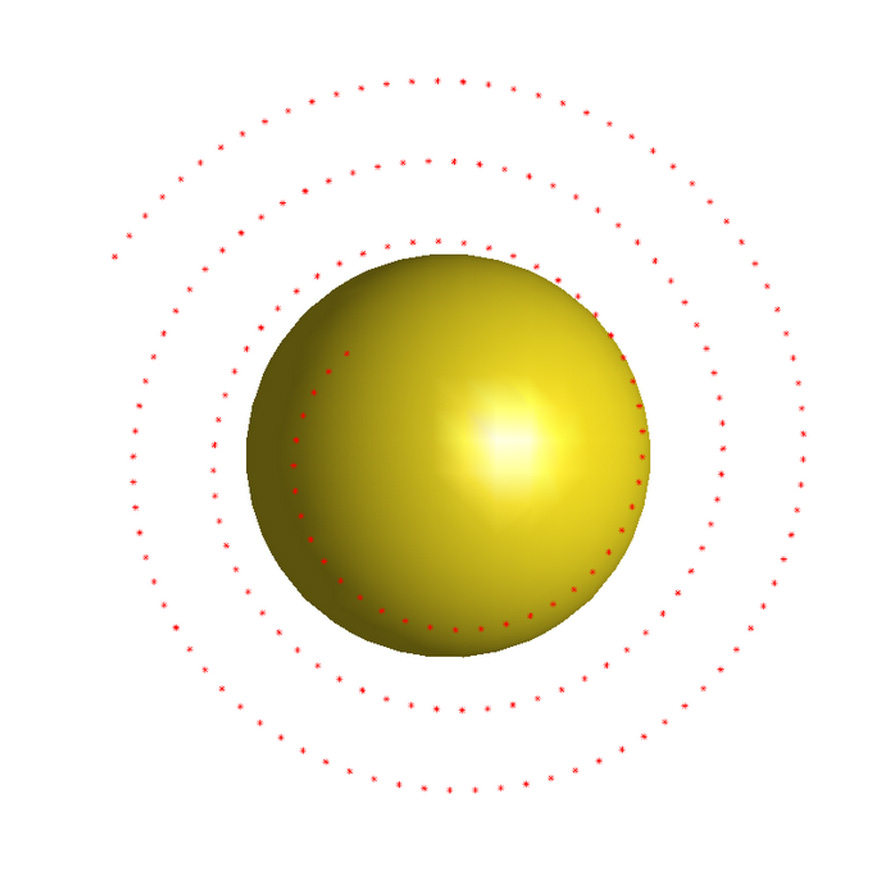
\includegraphics[scale=0.2]{eul2}
		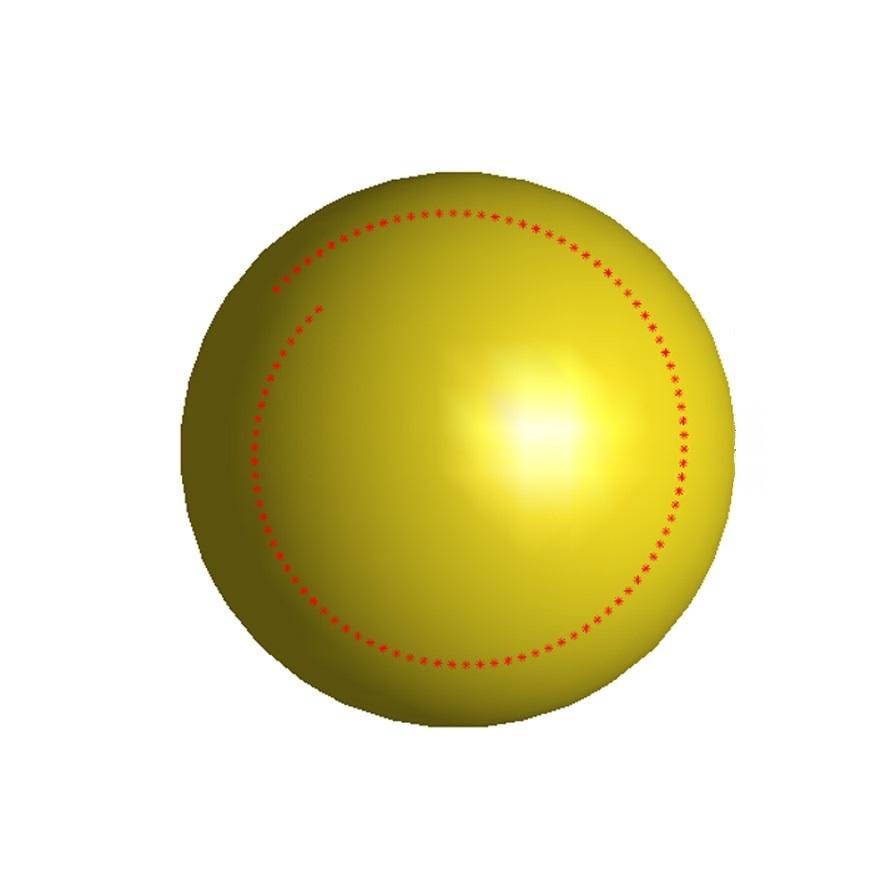
\includegraphics[scale=0.2]{eul1}
		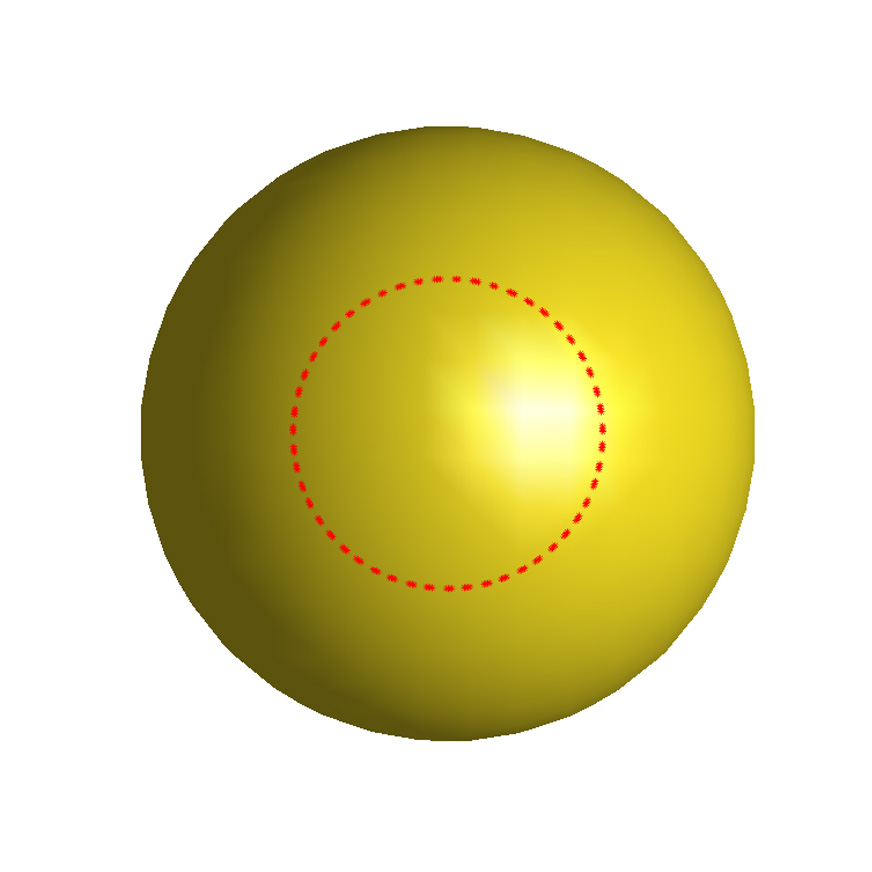
\includegraphics[scale=0.2]{eul3_newt}
		
	\end{frame}
	
	\begin{frame}{Potrebni pogoji in Jacobijeva matrika}
		Potreben pogoj za delovanje metod je, da sta funkciji $f_{1}$ in $f_{2}$ parcialno odvedljivi in da ima Jacobijeva matrika parcialnih odvodov poln rang 2. Za uspešno delovanje Newtonove metode moramo poiskati Jacobijevo matriko leve strani sistema nelinearnih enačb.
		
		\begin{center}
			JG = $\begin{bmatrix}
			grad(f_{1}) \\
			grad(f_{2}) \\
			grad(\vec{v} \cdot \vec{x}) \\
			\end{bmatrix}$
			oziroma
			JG = $\begin{bmatrix}
			grad(f_{1}) \\
			grad(f_{2}) \\
			\hspace{1mm}grad(\vec{v}\hspace{0.5mm}^\intercal) \\
			\end{bmatrix}$
		\end{center}
	\end{frame}
	
	\begin{frame}{Adaptivni korak}
	    Adaptivni korak nam omogoča bolj natančno rešitev problema. Deluje tako, da na vsakem koraku preveri čas, ki ga porabi za popravljanje napake z Newtonovo metodo in s tem podatkom ustrezno prilagodi velikost koraka.
	    
	    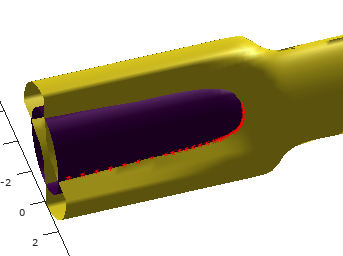
\includegraphics[scale=0.6]{slikaAda}
		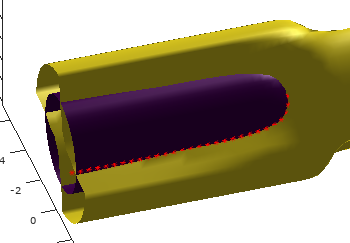
\includegraphics[scale=0.6]{slikaAda2}
		
	\end{frame}
	
	\begin{frame}{Končna analiza parov ploskev za vsak primer + slike}
		Delovanje našega programa lahko preverimo s programom, ki smo ga napisali v Octave-u. Kot vhodne parametre mu podamo obe implicitno podani funkciji $f_{1}$, $f_{2}$, $C1$, $C2$, $grad(f_{1})$, $grad(f_{2})$. Določimo tudi začetni približek $x_{0}$, začetno dolžino koraka in pa parameter, ki določa metodo delovanja (Euler/Runge-Kutta).
	\end{frame}
	
	\begin{frame}{Primer 1}
		Začnemo z preprostim primerom sfere in ravnine, podane z enačbama:\\
		
		\begin{itemize} 
			\item $f_{1}(x,y,z)$ = $x^2 + y^2 + z^2$ = 4
			\item $f_{2}(x,y,z)$ = $3x + 2y + z$ = 1	
		\end{itemize} 
		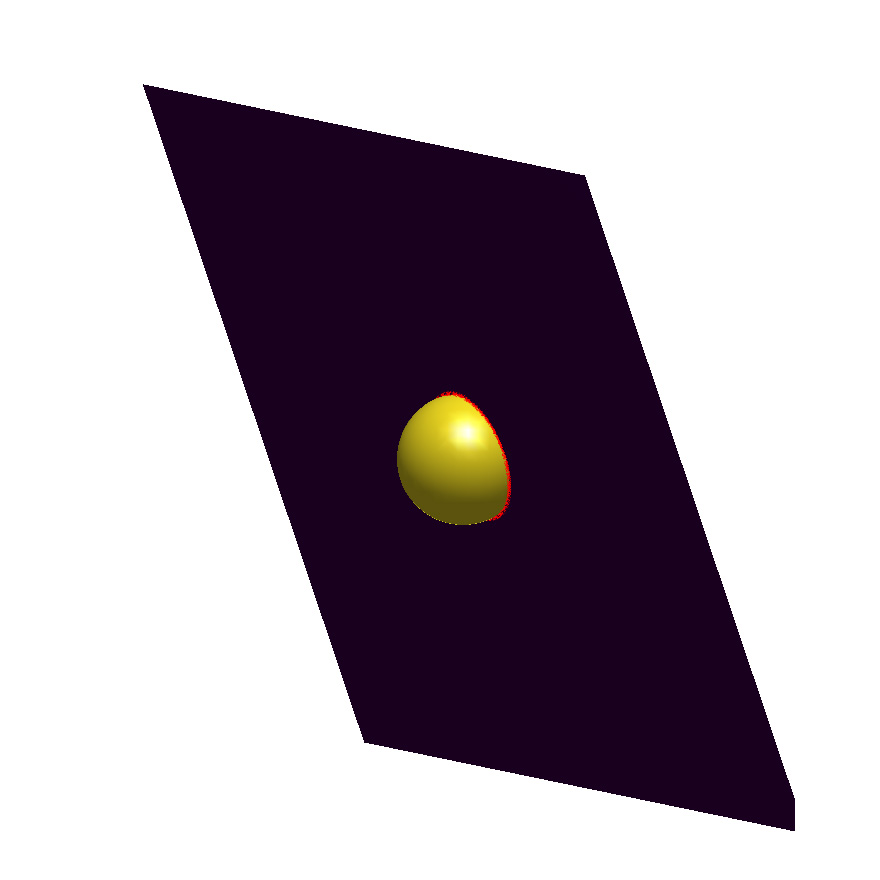
\includegraphics[scale=0.3]{primer1_1}
		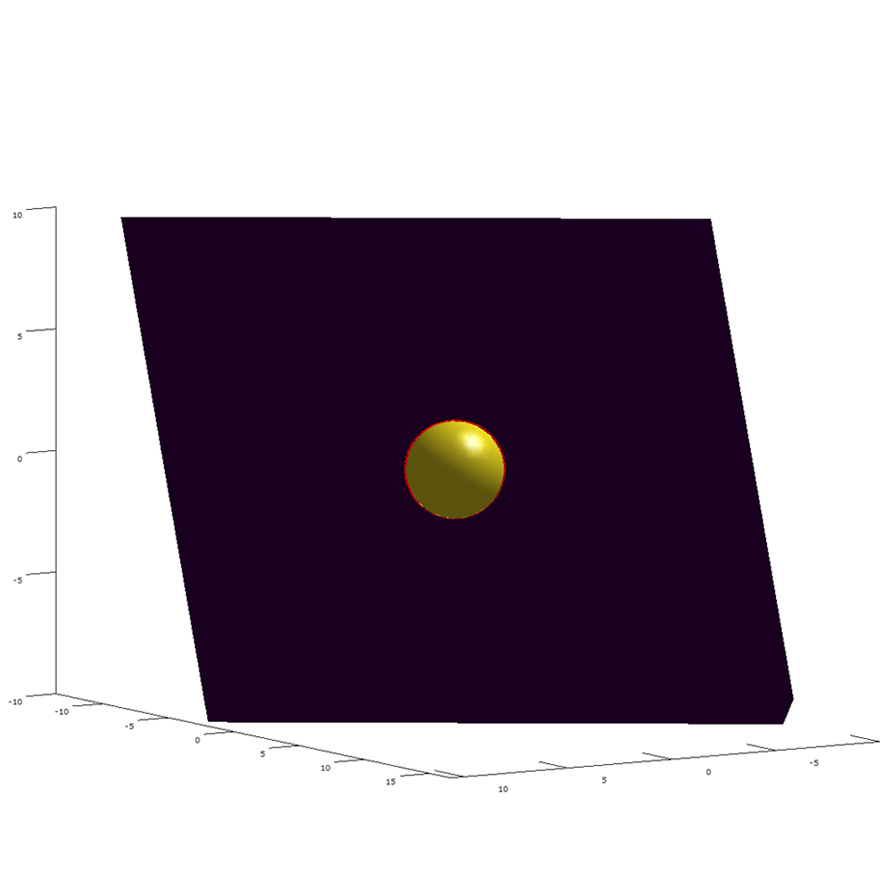
\includegraphics[scale=0.3]{primer1_2}
	\end{frame}
	
	\begin{frame}{Primer 2}
		Tudi primer sfere in valja je relativno "lep"\\
		
		\begin{itemize}  
			\item $f_{1}(x,y,z)$ = $x^2 + y^2 + z^2$ = 4
			\item $f_{2}(x,y,z)$ = $x^2 + y^2$ = 1
		\end{itemize} 
		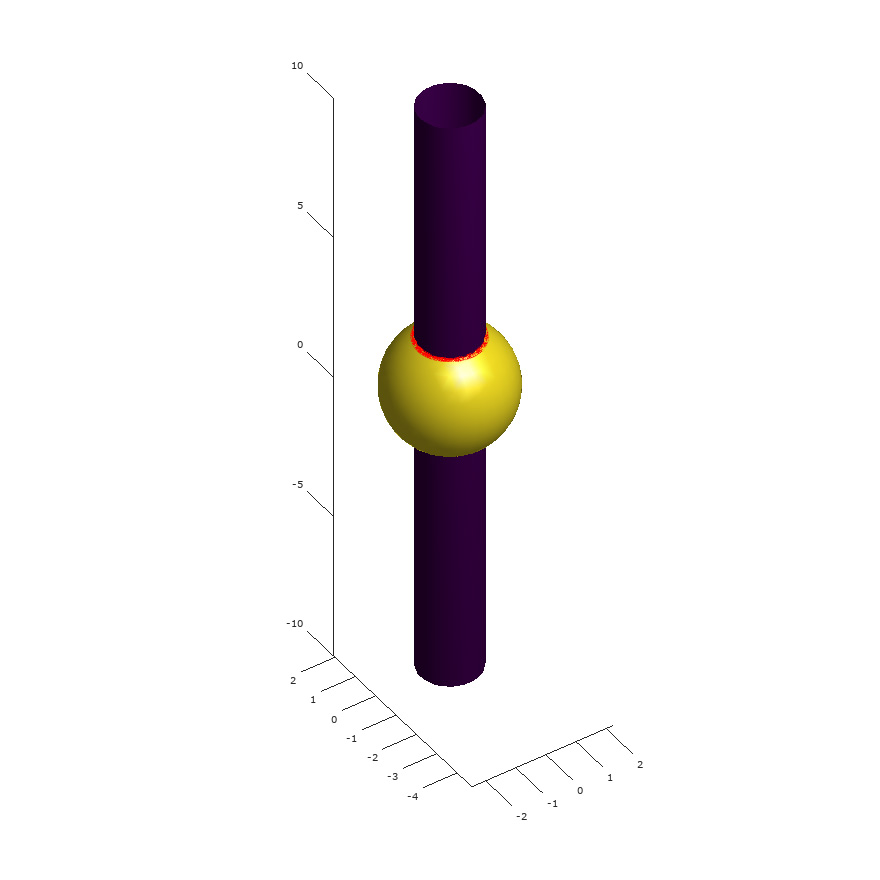
\includegraphics[scale=0.3]{primer2_1}
		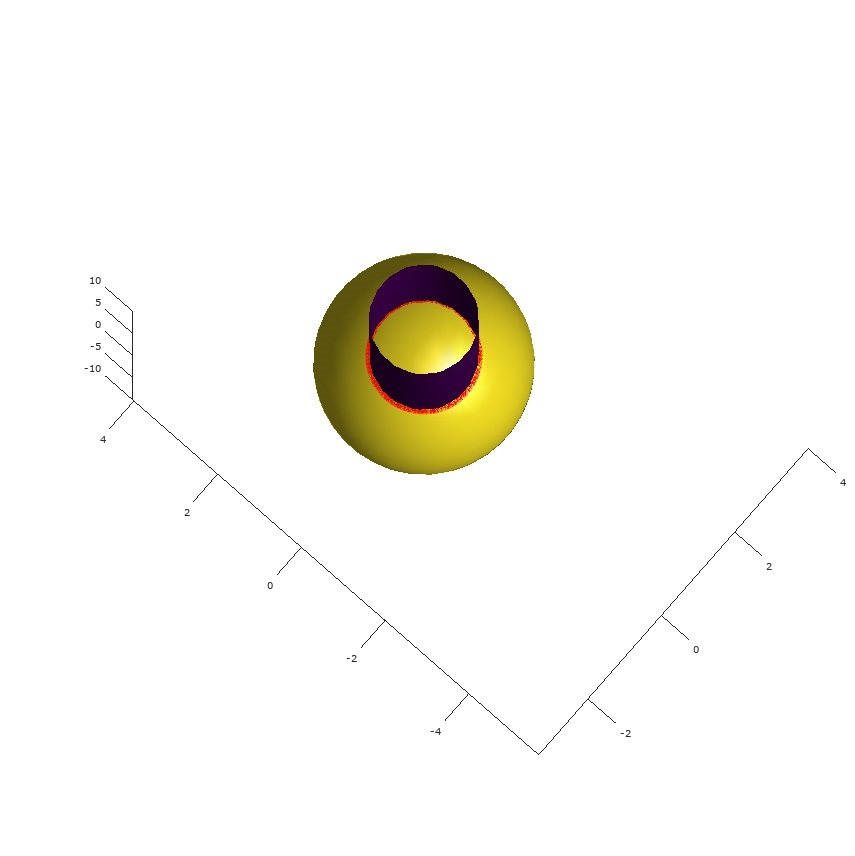
\includegraphics[scale=0.3]{primer2_2}
	\end{frame}
	
	\begin{frame}{Primer 3}
		Stvari malce otežimo s sfero in $f_{2}$
		
		\begin{itemize}  
			\item $f_{1}(x,y,z)$ = $x^2 + y^2 + z^2$ = 4
			\item $f_{2}(x,y,z)$ = $y^4 + log(x^2 + 1)z^2 - 4$ = 1
		\end{itemize} 
		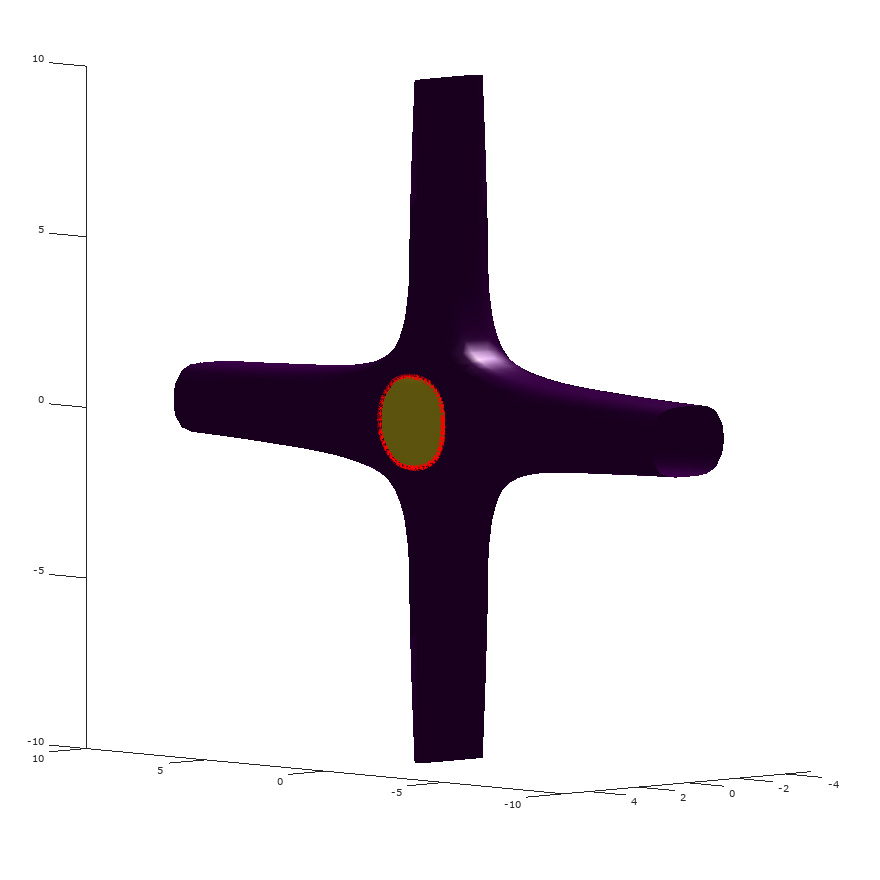
\includegraphics[scale=0.3]{primer3_1}
		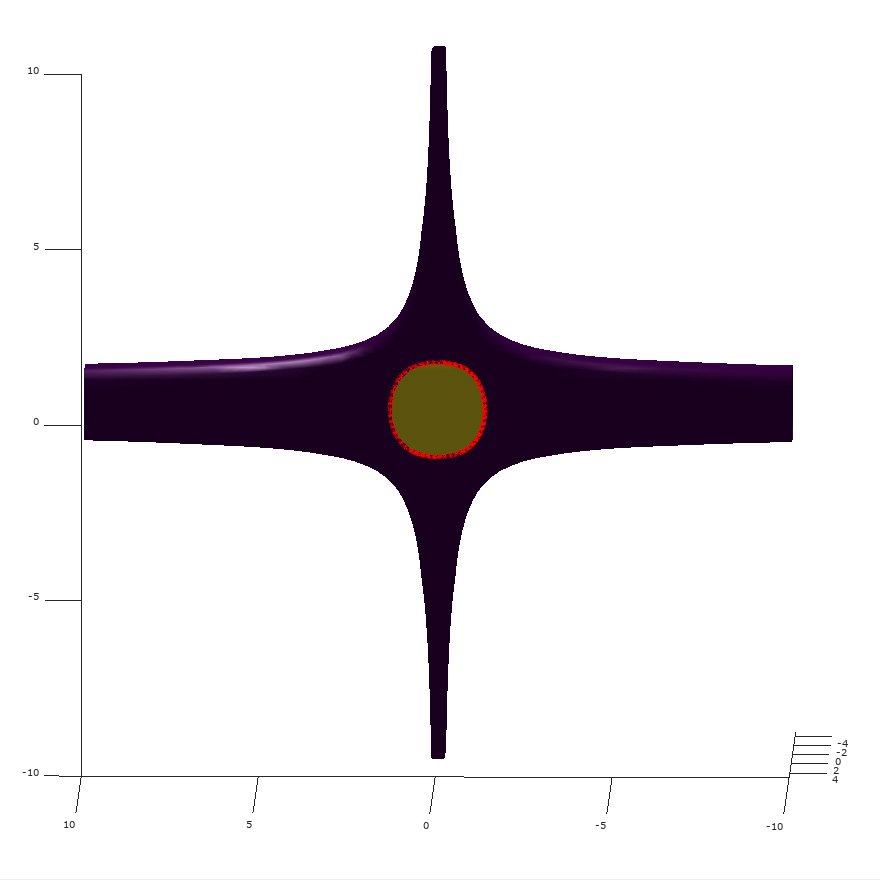
\includegraphics[scale=0.3]{primer3_2}
	\end{frame}
	\begin{frame}{Primer 4}
		
		\begin{itemize}  
			\item $f_{1}(x,y,z)$ = $x^2 + cos(y)z^2 - 12$ = 4
			\item $f_{2}(x,y,z)$ = $y^4 + log(x^2 + 1)z^2 - 4$ = 1
		\end{itemize} 
		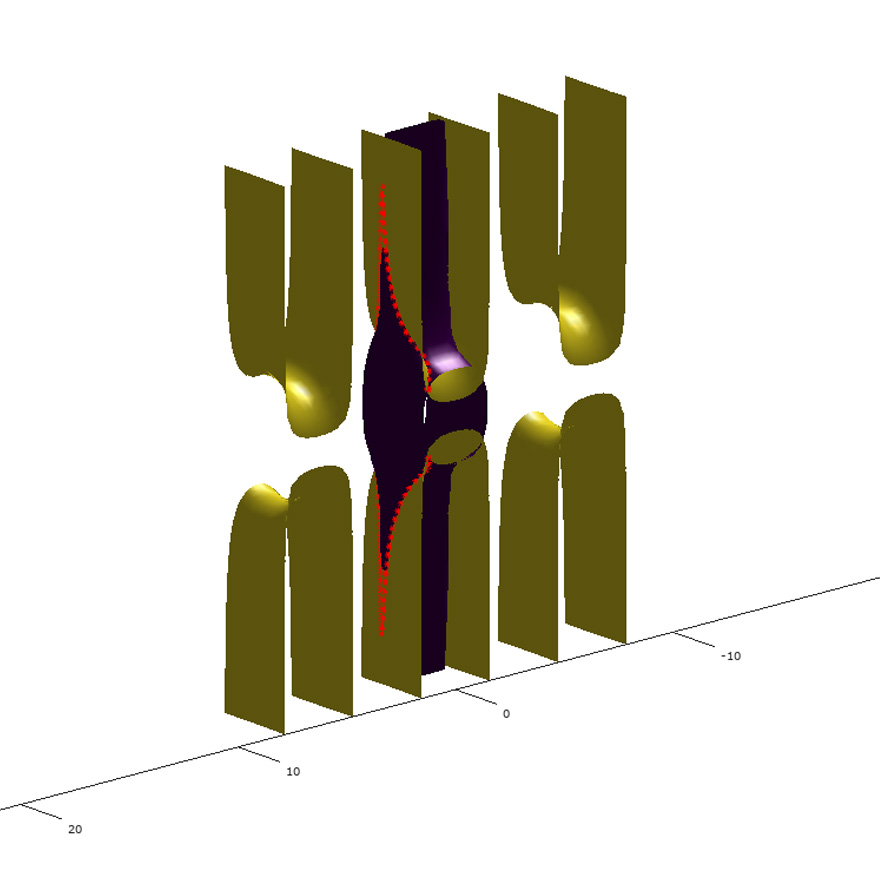
\includegraphics[scale=0.3]{primer4_1}
		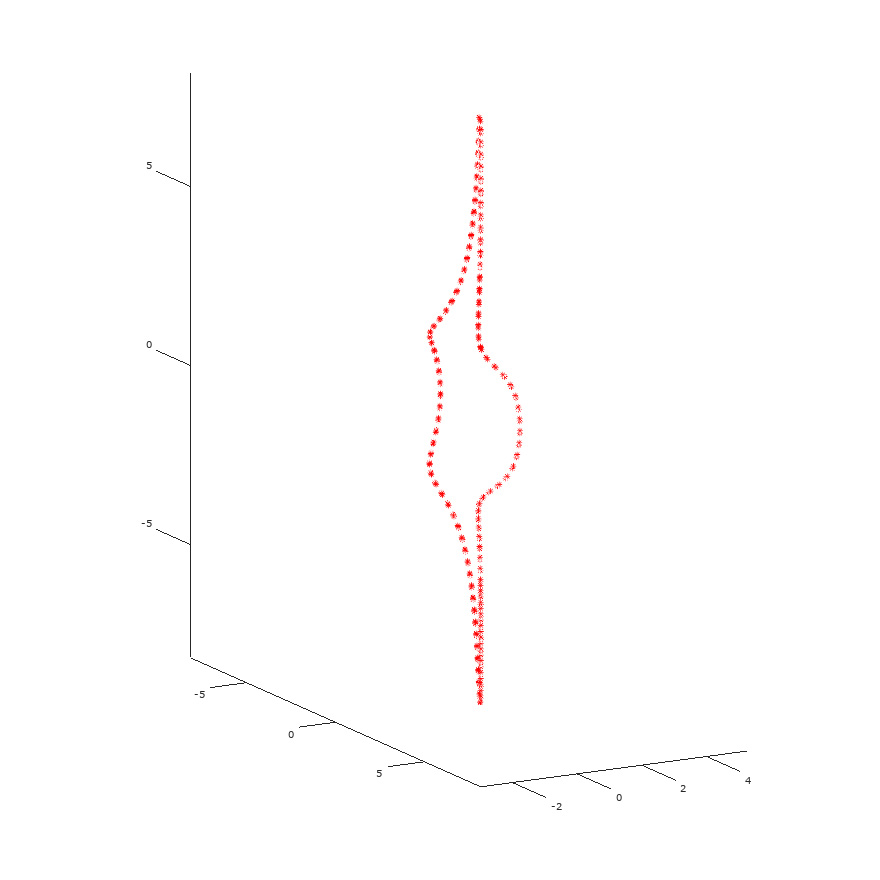
\includegraphics[scale=0.3]{primer4_4}
		
	\end{frame}
	
	\begin{frame}{Primer 4}
		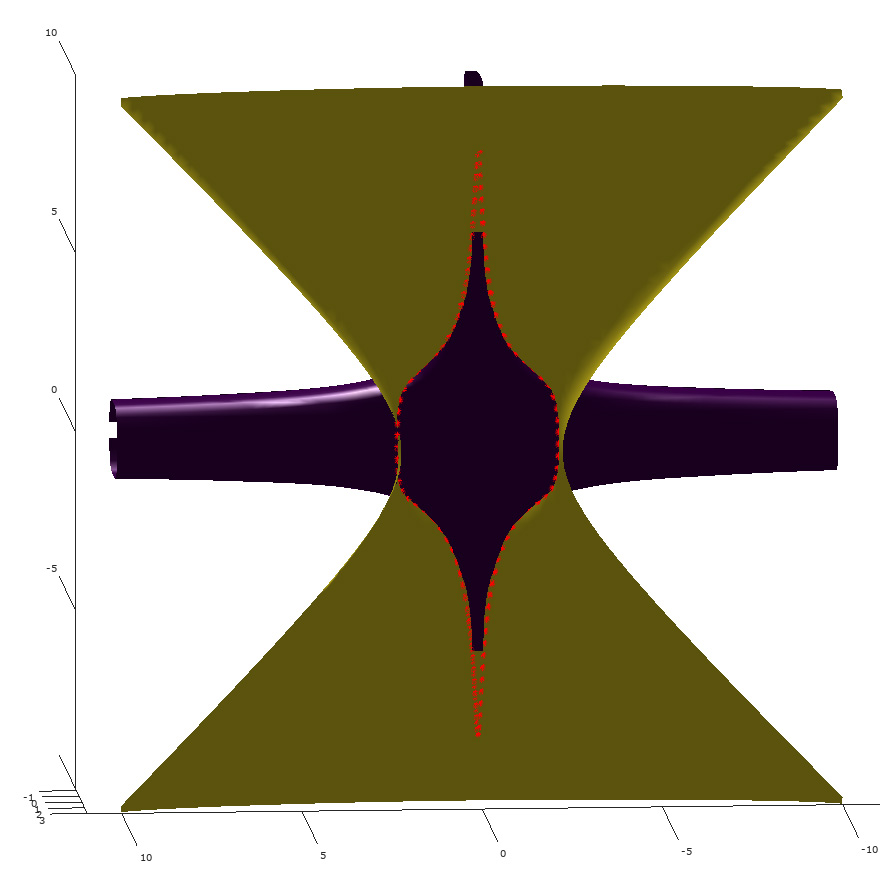
\includegraphics[scale=0.3]{primer4_2}
		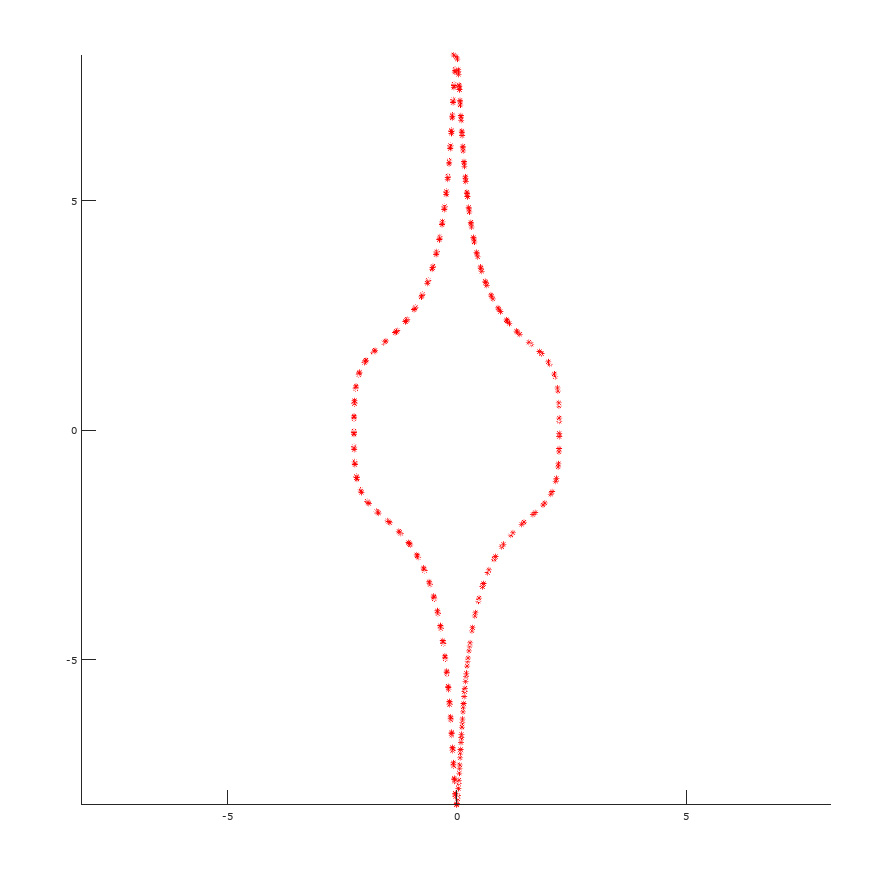
\includegraphics[scale=0.3]{primer4_3}
	\end{frame}
	
	\begin{frame}{Primer 5}
		\begin{itemize}  
			\item $f_{1}(x,y,z)$ = $e^{(-x^{2}+1)}+y^{2}+z^{2}$ = 3
			\item $f_{2}(x,y,z)$ = $e^{(xyz)}+y^{2}+z^{2}$ = 10
		\end{itemize} 
		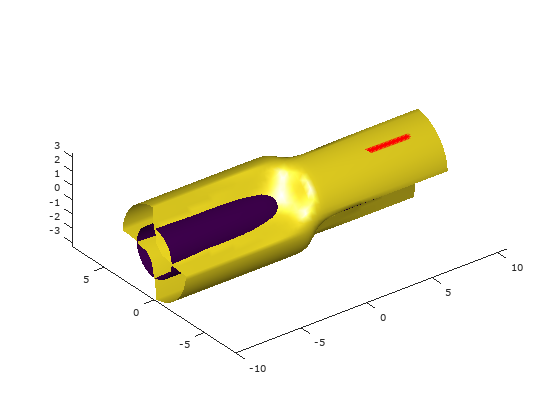
\includegraphics[scale=0.4]{primer5_1}
		%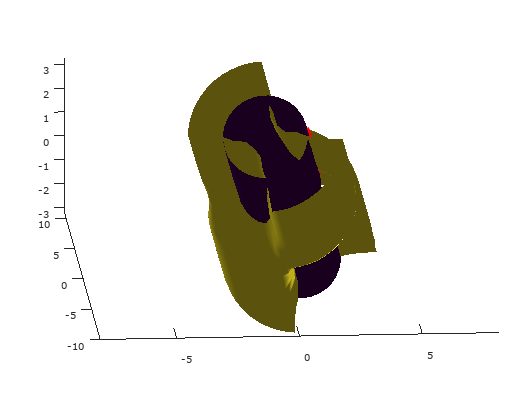
\includegraphics[scale=0.3]{primer5_2}
		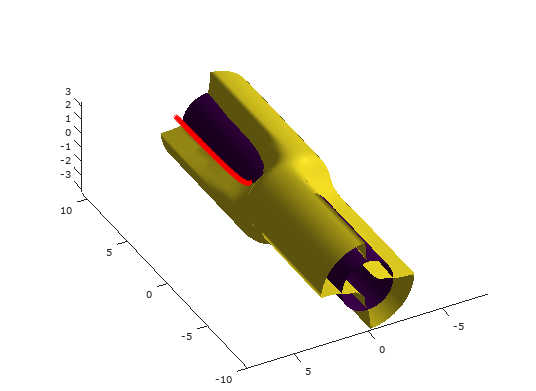
\includegraphics[scale=0.4]{primer5_4} 
	\end{frame}
	\begin{frame}{Primer 6}
		\begin{itemize}  
			\item $f_{1}(x,y,z)$ = $e^{(-x^{2}+1)}+y^{2}+z^{2}$ = 3
			\item $f_{2}(x,y,z)$ = $x^2 + y^2 + z^2$ = 4
		\end{itemize} 
		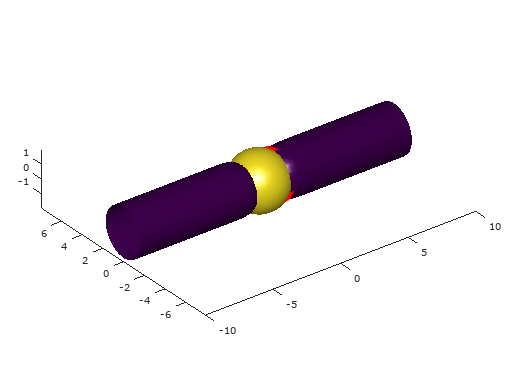
\includegraphics[scale=0.3]{primer6_1}
		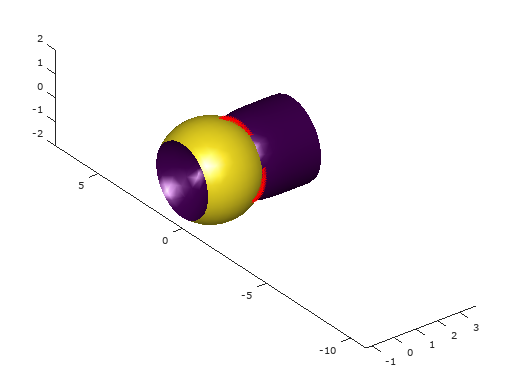
\includegraphics[scale=0.3]{primer6_2}
		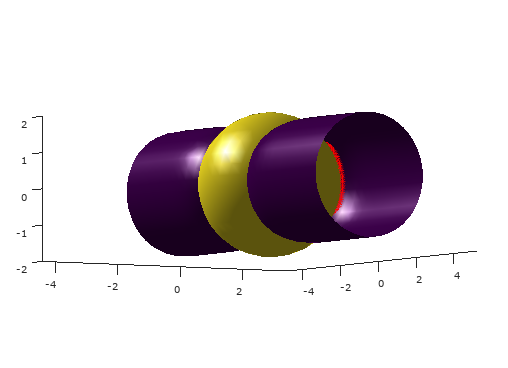
\includegraphics[scale=0.3]{primer6_3} 
	\end{frame}
	\begin{frame}{Primer 7}
		\begin{itemize}  
			\item $f_{1}(x,y,z)$ = $e^{(-x^{2}+1)}+y^{2}+z^{2}$ = 3
			\item $f_{2}(x,y,z)$ =  $x^2 + y^2$ = 1
		\end{itemize} 
		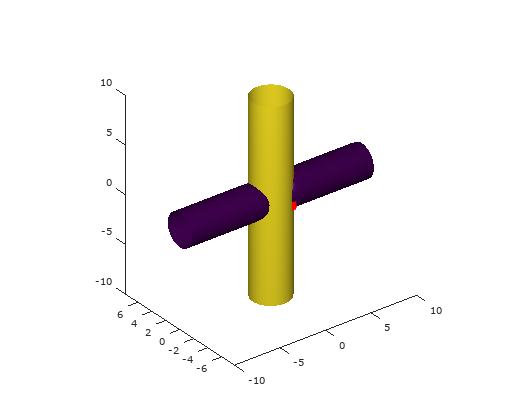
\includegraphics[scale=0.3]{primer7_1}
		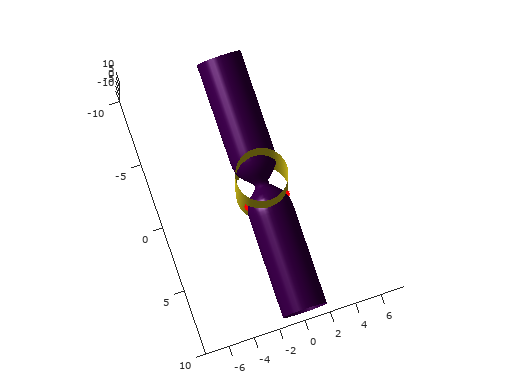
\includegraphics[scale=0.3]{primer7_2}
		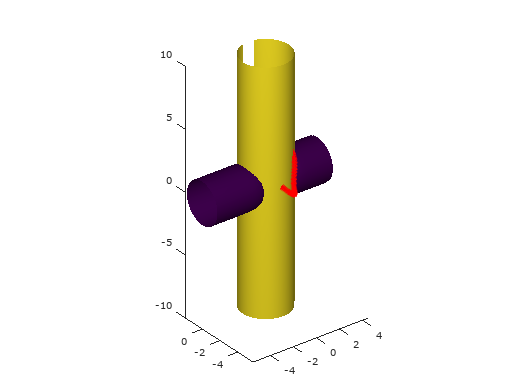
\includegraphics[scale=0.3]{primer7_3} 
	\end{frame}
	\begin{frame}{Primer 8}
		\begin{itemize}  
			\item $f_{2}(x,y,z)$ = $e^{(xyz)}+y^{2}+z^{2}$ = 10
			\item $f_{2}(x,y,z)$ =  $x^2 + y^2$ = 1
		\end{itemize} 
		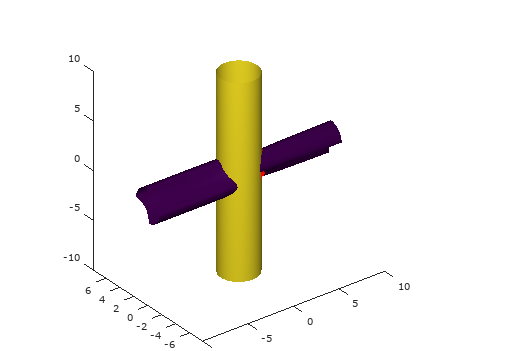
\includegraphics[scale=0.3]{primer8_1}
		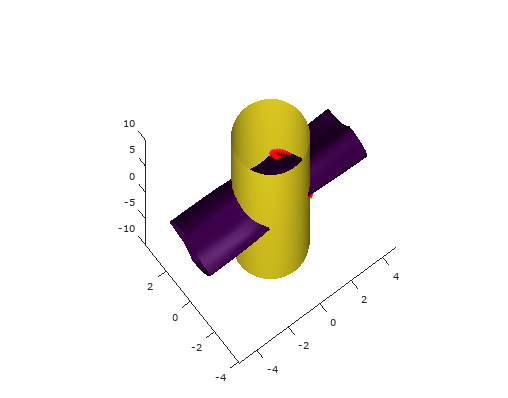
\includegraphics[scale=0.3]{primer8_2}
		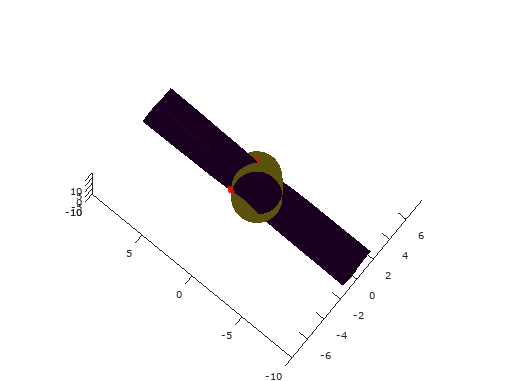
\includegraphics[scale=0.3]{primer8_3} 
	\end{frame}
	\begin{frame}{Analiza}
		Za vseh osem primerov smo naredili analizo, tako da smo izmerili povpre\v{c}no \v{s}tevilo korakov Newtonove metode z obe metode na dva na\v{c}ina: z adaptivnem in fiksnem koraku.
	\end{frame}
	\begin{frame}
 \begin{tabular}{|c | c | c | c | c |} 
 \hline
 \textbf{Funkcije} &\multicolumn{2}{|l|}{\textbf{Euler}} &\multicolumn{2}{|l|}{\textbf{RK4}}\\                
  \small &adaptivno & fiksno & adaptivno & fiksno \\ 
 \hline
 \tiny{}$f_{1}(x,y,z)=x^{2} + y^{2}+ z^{2}=4$ & & & &\\ 
 \tiny{}$f_{2}(x,y,z)=x^{2} + y^{2}    =1$  & 3 & 5 & 3 & 3.222 \\
 \hline
 \tiny{}$f_{1}(x,y,z)=x^{2} + y^{2}+ z^{2}=4$ & & & &\\ 
 \tiny{}$f_{2}(x,y,z)$ = $3x + 2y + z = 1$  & 3 & 4.222 & 3 & 3.333 \\
 \hline
 \tiny{}$f_{1}(x,y,z)=x^{2} + y^{2}+ z^{2}=4$ & & & &\\ 
 \tiny{}$f_{2}(x,y,z)$ = $y^4 + log(x^2 + 1)z^2 - 4 = 1$  & 3 & 5 & 3 & 3.222 \\
 \hline
 \tiny{}$f_{1}(x,y,z)$ = $x^2 + cos(y)z^2 - 12 = 4$ & & & &\\ 
\tiny{}$f_{2}(x,y,z)$ = $y^4 + log(x^2 + 1)z^2 - 4 = 1$  & 3 & 4.111 & 2.222 & 2.556 \\
 \hline
 \tiny{}$f_{1}(x,y,z)$ = $e^{(-x^{2}+1)}+y^{2}+z^{2} = 3$ & & & &\\ 
 \tiny{}$f_{2}(x,y,z)$ = $e^{(xyz)}+y^{2}+z^{2} = 10$  & 3 & 4.667 & 2.222 & 2.667 \\
 \hline
 \tiny{}$f_{1}(x,y,z)$ = $e^{(-x^{2}+1)}+y^{2}+z^{2} = 3$ & & & &\\ 
 \tiny{}$f_{2}(x,y,z)=x^{2} + y^{2}+ z^{2}=4$  & 3 & 5 & 3 & 3.222 \\
 \hline
 \tiny{}$f_{1}(x,y,z)$ = $e^{(-x^{2}+1)}+y^{2}+z^{2} = 3$ & & & &\\ 
  \tiny{}$f_{2}(x,y,z)=x^{2} + y^{2}    =1$  & 3 & 5 & 3 & 3.333 \\
  \hline
\tiny{}$f_{1}(x,y,z)$ = $e^{(xyz)}+y^{2}+z^{2} = 10$ & & & &\\ 
 \tiny{}$f_{2}(x,y,z)=x^{2} + y^{2}    =1$  & 3 & 5 & 3 & 3.556 \\
  \hline
\end{tabular}
	\end{frame}
	
\end{document}
